% This creates a document based on the AMS
% (American Mathematical Society) article style.
\documentclass[11pt]{article}

% This package simply sets the margins to be 1.00 inch.
% If you prefer 1.25 in margins change the value.
% If you look up the documentation for the geometry package
% you can find out how to control the size of all four margins
% independently of each other.
\usepackage[margin=1.00in]{geometry}

% These packages include nice commands from AMS-LaTeX
% AMS-LaTeX has lots of nice equation environment that are better
% than the plan LaTeX options.
\usepackage{amssymb,amsmath,amsthm, enumitem, bm, graphicx, mathrsfs, bbm}

% Make the space between lines slightly more
% generous than normal single spacing, but compensate
% so that the spacing between rows of matrices still
% looks normal.  Note that 1.1=1/.9090909...
\renewcommand{\baselinestretch}{1.1}
\renewcommand{\arraystretch}{.91}
% If you want even more space between lines try
% \renewcommand{\baselinestretch}{1.5}
% \renewcommand{\arraystretch}{0.67}

% Define a new environment for exercises.
\newenvironment{exercise}[1]{\vspace{.1in}\noindent\textbf{Exercise #1 }}{}

% Define shortcut commands for commonly used symbols.
\newcommand{\R}{\mathbb{R}} % Real numbers
\newcommand{\C}{\mathbb{C}} % Complex numbers
\newcommand{\Z}{\mathbb{Z}} % Integers
\newcommand{\Q}{\mathbb{Q}} % Rational numbers
\newcommand{\N}{\mathbb{N}} % Natural numbers
\newcommand{\calP}{\mathcal{P}} % Calligraphic P for power set
\newcommand{\calN}{\mathcal{N}}
\newcommand{\calR}{\mathcal{R}}
\newcommand{\F}{\mathbb{F}} % Field
\newcommand{\E}{\mathbb{E}} % Expected Value

\newcommand{\unif}{\text{Uniform}} 
\newcommand{\normaldist}{\mathcal{N}} 
\newcommand{\gammadist}{\text{Gamma}} 
\newcommand{\empirical}{\text{Emp}} 
\newcommand{\argmax}{\text{ArgMax}} 
\newcommand{\argmin}{\text{ArgMin}} 
\newcommand{\pdf}{f} 
\newcommand{\given}{|} 
\newcommand{\KL}{\mathbb{KL}} 

% vectors and subspaces
\renewcommand{\vec}[1]{{\ensuremath{\bm{#1}}}}
\newcommand{\0}{{\vec  0 }}
\newcommand{\1}{{\mathbbm{  1} }}
\newcommand{\J}{{\vec  J }}
\renewcommand{\a}{{\vec  a }}
\renewcommand{\b}{{\vec  b }}
\renewcommand{\c}{{\vec  c }}
\renewcommand{\d}{{\vec  d }}
\newcommand{\e}{{\vec  e }}
\newcommand{\f}{{\vec  f }}
\newcommand{\g}{{\vec  g }}
\newcommand{\h}{{\vec  h }}
\renewcommand{\k}{{\vec  k }}
\renewcommand{\l}{{\boldsymbol{\ell} }}  % lowercase l looks too much like 1.  
\newcommand{\m}{{\vec  m }}
\newcommand{\p}{{\vec  p }}
\newcommand{\q}{{\vec  q }}
\renewcommand{\r}{{\vec  r }}
\newcommand{\s}{{\vec  s }}
\renewcommand{\t}{{\vec  t }}
\let\uaccent\u
\renewcommand{\u}{{\vec  u }}
\let\vaccent\v
\renewcommand{\v}{{\vec  v }}
\newcommand{\w}{{\vec  w }}
\newcommand{\x}{{\vec  x }}
\newcommand{\y}{{\vec  y }}
\newcommand{\z}{{\vec  z }}
\newcommand{\bZ}{{\vec{Z}}}
\newcommand{\X}{{\mathbb{X}}}
\renewcommand{\L}{{\mathscr{L}}}

% Define a function called "span" that would be useful in linear algebra.
\DeclareMathOperator{\vsspan}{span}

% Define functions for the real and imaginary parts of a complex number.
% These could be used in place of the built in commands \Re and \Im,
% which print Re and Im in a font that some people don't like.
\DeclareMathOperator{\re}{Re}
\DeclareMathOperator{\im}{Im}



%%%%%%%%%%%%%%%%%%%%%%%%%%%%%%%%%%%%%%%%%%

\begin{document}
    
    % If you use Overleaf, the name of the project will be determined by
    % what you enter as the document title.
    \title{Recognizing Spoken Arabic Numerals}
    \author{Calix Barrus, Dallan Olsen, Elijah Cox, Laren Edwards}
    
    \maketitle
    
    \begin{abstract}
        Do the same principles used in English language recognition apply to other languages? This project sets out to use typical methods of speech recognition for the English language on Arabic speakers saying numbers 0 to 9. A Gaussian Mixture Model Hidden Markov Model is used for each digit and is compared to a UMAP dimensionality reduction paired with a KMeans classifier. We then compare results to see if GMMHMMs work as well in identifying Arabic words as they do English words.
    \end{abstract}
    
    \section{Problem Statement and Motivation}
    Speech recognition is a big part of many of the technologies around us, from our phones to our homes. It can simplify our lives and make information much easier to capture and send. Most of the research, though, has been centered on speech recognition in the English language. A significantly smaller amount of research has been dedicated to other languages. The question is, do the same principles used in English language recognition apply to other languages? Research done in “Speech Recognition of Moroccan Dialect Using Hidden Markov Models” \cite{RefWorks:RefID:42-mouaz2019speech} notes that more work needs to be done to recognize words spoken in Arabic since there are so many dialects. Typical methods used for English just don’t work as well, and it is only after identifying the dialect of the speaker that the speaker’s words can be accurately classified. Another paper, “Application of Hidden Markov Models in Speech Command Recognition” \cite{RefWorks:RefID:41-2020application}, noticed that model accuracy was much lower than normal when trying to identify Chinese phrases with typical methods used in the English language. Therefore, this project seeks to expand on how well HMMs and other classifiers work with speech recognition in languages other than English. For this project, we will be analyzing sound files of native Arabic speakers speaking the numbers 0 through 9. We will then test our model against a test dataset to see if we can determine which number is being spoken and the gender of the speaker. 
    
    \section{Data}
    Our data came from the database, “Spoken Arabic Digits” and was produced by the Laboratory of Automatic and Signals, University of Badji-Mokhtar, Annaba, Algeria. The dataset contains 8800 (10 digits x 10 repetitions x 88 speakers) time series of 13 Frequency Cepstral
    Coefficients (MFCCs). The speakers chosen are 44 males and 44 females who are Arabic native speakers between the ages 18 and 40. Each one repeated each digit 10 times. The data has already been split into a training set and a test set with the training set having 6600 utterances and the test set containing 2200. The training set has 33 male speakers and 33 female speakers. Each utterance is split into blocks of MFCCs. The first 660 blocks represent the digit zero with the first 330 being spoken by our 33 males and the last 330 being spoken by our 33 females. The blocks continue in this manner with blocks 661-1320 being the digit one, and so on until digit nine. The test set is divided similarly, but in sets of 220 blocks with the first 110 being spoken by 11 remaining male speakers and the next 110 being from our 11 remaining female speakers. 
    
    \section{Methods}
    We are using a set of Gaussian Mixture Model Hidden Markov Models (GMMHMMs) to classify both the digit said and the gender of the speaker. We chose this because it is a good model for classifying time series data when we know what the possible classifications are and when we have known observations of these classifications. We compare the success of this method to a UMAP dimensional reduction, paired with a k-nearest neighbors classifier.
    For the formulation of our UMAP classifier, we truncated the data from each utterance to be uniform throughout the dataset. Because the shortest utterance was only four rows of MFCC, (these ranged from 4 - 90+ rows of MFCCs per utterance) we only considered the first four rows of each utterance for both the training and test sets. The next step was to perform the actual dimensionality reduction, which we did using UMAP to a 2-dimensional space. This resulted in an effective visualization of the data. After creating the dimensionality reduction function using UMAP, we transformed all the data through the function and visualized it. Then, using information about the training set, we used a SciKitLearn’s k-nearest neighbors implementation to classify the data points from the test set.
    
    \section{Results}
    The UMAP training took less than a minute for all 6600 training set observations, which is admirable performance. For the KNN classifier, we used the 100 nearest neighbors to classify the test set. Observing the visualizations, it seems plausible that this is a valid (though imperfect) method for classifying the data points. We see that this is indeed the case; this strategy had 81\% accuracy for gender classification, and an impressive 64\% accuracy for digit classification. This is much better than random (10\%) and is a useful baseline to compare our GMMHMM against. 
    
    The GMMHMM itself is currently unable to quite match the performance of the baseline UMAP clustering, achieving 58\% accuracy on the test set. However, a single data processing complication prevents it from being fully exploited, and we believe this alone may be preventing the GMMHMM from outperforming the baseline. The blocks of MFCCs are of variable length, and we keep only a uniform amount of rows so that the MFCC can be trained. This may inhibit its performance.
    
    Looking at the resulting visualization, we can see that UMAP does a decent job for many of the digits. For some of the digits, especially 9 and 5 have their own clear space clusters in the resulting mapping. 
    
    
    \begin{figure}
        \centering
        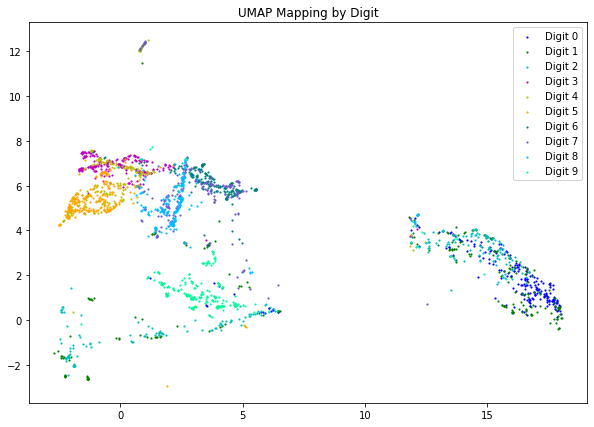
\includegraphics[width=0.7\linewidth]{UMAPdigitcomparison}
        \caption{}
        \label{fig:umapdigitcomparison}
    \end{figure}
    
    
    Coloring points by gender, we can also see that the UMAP mapping separates males and females into distinct groups in most cases. 
   
    \begin{figure}
        \centering
        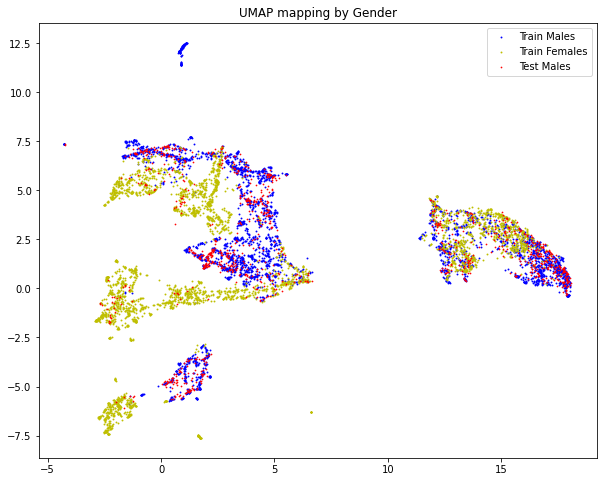
\includegraphics[width=0.7\linewidth]{UMAPGenderCompare}
        \caption{}
        \label{fig:umapgendercompare}
    \end{figure}
    
    \section{Analysis}
    
    \subsection{UMAP}
    Our results using UMAP and K Nearest Neighbors were much better than expected, especially given the limited data we used (we truncated the data). Furthermore, the UMAP technique doesn’t take into account all the time series nature of the data, as the whole time series is just considered as some d-dimensional data point. Finally, UMAP was much easier to implement, compared to our initial experiences with GMMHMM, which doesn’t (usually) build expectations of good performance. Despite these factors, our UMAP technique did much, much better than random. 
    
    In addition, it is worth pointing out that the technique used by the UMAP library to predict mappings of additional data points seems to be quite effective. Looking at the Figure \ref{fig:umapgendercompare}, it seems clear that the males in the test data were generally mapped very close to males in the training data. This provides strong evidence that the UMAP does a good job at predicting where the new data points will lie in the reduced dimensional space. This is significant since accounting for new data points is considered a weakness of nonlinear dimension reduction techniques (or so we thought), but this implementation does an excellent job at shoring up that supposed weakness. 
    
    \subsection{GMMHMM}
    Our implementation and use of GMMHMM on this problem is in theory much better suited to the nature of the data. GMMHMMs have a lot of flexibility and by combining many different gaussian distributions in different combinations and sequences, they can be used to describe many types of patterns in high dimensional data. A particular feature of GMMHMMs that lend themselves towards this particular problem is their ability to use temporal information. Since each Gaussian HMM has state transition going on behind the scenes, they are very much able to recognize and use temporal relationships in data. This feature leads us to expect that GMMHMMs will be able to perform well at this task of language recognition. 
    Our initial results with GMMHMMs suggest a measure of careful optimism that, with more time and training and using more of the data our GMMHMMs will perform better and better. 
    
    \section{Ethical Considerations}
    There are several ethical considerations for the use and misuse of this technique. It could be used to spy on and censor people in Arab countries. In the hands of the wrong people, it could be used to control people with devastating effects.. If used maliciously, it could be a vehicle for political control. 
    % add in good ethical stuff on low resource languages
    
    \section{Conclusion}
    For now, it seems that using UMAP to reduce the dimensionality of the data and then using a KMeans clustering algorithm classifies more accurately than a GMMHMM. However, in order to pass the data into a GMMHMM, we took only 4 rows of MFCC’s. This means that a lot of information was lost and thus, our classifier did not perform as well. The next step is to either adapt our GMMHMM to take arrays of variable length or to use some kind of function to transform all our data so that they have the same size. So, for now, we cannot conclude definitively that GMMHMMs do not work for Arabic and further analysis will need to be done.
    

    
    %---------------------------------
    % Don't change anything below here
    %---------------------------------
    
\bibliographystyle{plain}
\bibliography{export}    
    
\end{document}
